\documentclass{article}

\usepackage[utf8]{inputenc}
\usepackage[T1]{fontenc}
\usepackage{hyperref}
\usepackage{url}
\usepackage{booktabs}
\usepackage{amsfonts}
\usepackage{amsmath}
\usepackage{amssymb}
\usepackage{graphicx}
\usepackage{microtype}
\usepackage[numbers]{natbib}
\usepackage{multirow}
\usepackage{amsthm}
\usepackage{algorithm}
\usepackage{algpseudocode}
\usepackage[margin=1in]{geometry}
\usepackage{float}
\usepackage{array}
\usepackage{xcolor}

\newtheorem{theorem}{Theorem}
\newtheorem{definition}{Definition}
\newcommand{\tx}{\ensuremath{\times}}

\hypersetup{
    colorlinks=true,
    linkcolor=blue,
    urlcolor=cyan,
    citecolor=blue,
    pdftitle={Decoupled Shelf Routing for Multi-Cobot Warehouses},
}

\title{Decoupled Shelf Routing for Multi-Cobot Warehouses: A Two-Layer Integration of VRP-RPD and Multi-Agent Path Finding}



\date{\today}

\begin{document}

\maketitle

% ============================================================
\begin{abstract}

Autonomous mobile robots in warehouse operations must deliver shelf units to
workstations, allow processing to complete, and retrieve the shelves for
redeployment, all while sharing a common grid network. Task assignment, route
sequencing, and collision avoidance on the grid must be solved jointly because
solutions to each subproblem constrain the others. Commercial goods-to-person
systems assign both delivery and retrieval of each shelf to the same robot,
requiring the robot to wait at the workstation throughout processing and limiting
the number of shelves in simultaneous processing to the fleet
size~\cite{kiva_patent_2014}. Multi-agent pickup and delivery formulations
impose the same single-agent-per-task constraint~\cite{ma2017lifelong}. We build
on the Vehicle Routing Problem with Resource-Constrained Pickup and Delivery
(VRP-RPD)~\cite{vrp_rpd_gecco_2026}, which permits any robot to retrieve a
shelf regardless of which robot delivered it, and extend it to multiple depots
and stochastic processing times. We propose a two-layer architecture in which
VRP-RPD plans task assignments and route sequences while a Multi-Agent Path
Finding (MAPF) solver computes collision-free paths on the warehouse grid. An
iterative coupling step propagates MAPF-induced traversal delays back to VRP-RPD
as updated edge weights, triggering replanning when delays alter solution
feasibility. Experiments on a physical testbed of 5--6 cobots operating over a
100-node grid with multiple depots show that cross-agent retrieval outperforms
same-agent round trips when the ratio of mean processing time to mean travel time
exceeds a threshold determined empirically, and that iterative coupling reduces
makespan relative to treating the two layers independently.

\end{abstract}

% ============================================================
\section{Introduction}

In goods-to-person warehouse operations, mobile robots retrieve shelf units from
storage, transport them to workstations where tasks are performed, and return
the shelves to storage. The Amazon Robotics system assigns both delivery and
retrieval of each shelf to the same robot; the robot waits at the workstation
throughout the task before returning the shelf~\cite{kiva_patent_2014}. Each
robot is therefore unavailable for other assignments for the full duration of
processing, and the number of shelves in simultaneous processing is bounded by
fleet size.

When processing time exceeds travel time, a waiting robot is not executing
transport. Releasing a robot after shelf delivery and assigning retrieval to
whichever robot is available when processing completes removes this bound. The
number of shelves in active processing is then independent of fleet size,
determined instead by the rate at which robots deliver.

The Vehicle Routing Problem with Resource-Constrained Pickup and Delivery
(VRP-RPD)~\cite{vrp_rpd_gecco_2026} formalizes this model. A fleet of vehicles
carries finite identical resources to customer locations, each resource processes
autonomously for a fixed duration, and any vehicle may perform retrieval
regardless of which vehicle performed delivery. VRP-RPD is computationally
intractable beyond 16 customers~\cite{vrp_rpd_gecco_2026}. A sequential
ALNS$\to$BRKGA metaheuristic pipeline reduces makespan by up to 74\% over
baselines on TSPlib-derived benchmarks with up to 1000 nodes~\cite{vrp_rpd_gecco_2026}.

We extend VRP-RPD in three directions. First, shelves and robots originate from
multiple depots distributed across the warehouse floor. Second, processing times
are stochastic, reflecting variable task durations. Third, robots share a
physical grid network where aisle segments have limited capacity, requiring
collision and deadlock avoidance. VRP-RPD treats travel times as fixed scalars
and does not represent route interactions on the grid.

We propose a two-layer architecture. VRP-RPD assigns shelves to robots and
sequences deliveries and retrievals to minimize expected makespan. A
Multi-Agent Path Finding (MAPF) solver then computes collision-free paths for
each robot on the warehouse grid. When MAPF introduces wait steps to resolve
conflicts, effective edge traversal times increase beyond VRP-RPD's assumed
values. These delays may push pickup times past processing completion, alter
delivery and retrieval ordering, and render the VRP-RPD solution infeasible.
Treating the two layers as independent ignores these interactions. We propose an
iterative coupling in which MAPF-induced delays are fed back to VRP-RPD as
updated edge weights, triggering replanning until the two layers produce a
consistent solution.

\textbf{Contributions.}
\begin{enumerate}
    \item We extend VRP-RPD to multiple depots and stochastic processing times,
    producing a formulation applicable to physical warehouse cobot systems.
    \item We propose an iterative two-layer VRP-RPD/MAPF architecture with a
    feedback mechanism that propagates execution-layer delays to the planning
    layer.
    \item We identify the ratio of mean processing time to mean travel time as
    the parameter governing when cross-agent retrieval reduces makespan relative
    to same-agent round trips, and determine the crossover value experimentally.
    \item We validate the architecture on a physical testbed of 5--6 cobots
    operating on a 100-node warehouse grid with multiple depots.
\end{enumerate}

Section~\ref{sec:related} reviews related work. Section~\ref{sec:problem}
defines the extended VRP-RPD. Section~\ref{sec:method} presents the two-layer
architecture. Section~\ref{sec:experiments} describes experiments.
Section~\ref{sec:conclusion} concludes.

% ============================================================
\section{Related Work}
\label{sec:related}
% ============================================================

\subsection{Goods-to-Person Warehouse Systems}

The Amazon Robotics system assigns delivery and retrieval of each shelf to the
same mobile drive unit (MDU); the MDU waits at the picking station throughout
the operation before returning the shelf to storage, as described in its patent
documentation~\cite{kiva_patent_2014}. Robot utilization is therefore coupled
to workstation processing time. Work on order assignment and station scheduling
in this system~\cite{kiva_order_scheduling} optimizes throughput within the
same-agent constraint but does not relax it. The collaborative scheduling
problem for heterogeneous robots (CSHR-SPD)~\cite{cshr_spd_2025} introduces a
three-stage ACR--AMR--ACR structure with a makespan objective. CSHR-SPD pairs
the same robot type for delivery and retrieval and does not permit cross-agent
pickup.

\subsection{Vehicle Routing Problem with Resource-Constrained Pickup and Delivery}

VRP-RPD~\cite{vrp_rpd_gecco_2026} permits any vehicle to retrieve a resource
regardless of which vehicle delivered it, without requiring intermediate
transfer points. Classical pickup-and-delivery problems require the same vehicle
for both operations~\cite{berbeglia2007static, parragh2010variable}. VRP-RPD
was shown to be NP-hard, and an ALNS$\to$BRKGA pipeline produces the best
known results on TSPlib-derived benchmarks~\cite{vrp_rpd_gecco_2026}. The
present work extends VRP-RPD to multiple depots, stochastic processing times,
and a grid network with spatial conflicts.

\subsection{Multi-Agent Path Finding}

Multi-Agent Path Finding (MAPF) finds collision-free, deadlock-free paths for a
set of agents on a graph~\cite{stern2019multi}. The Multi-Agent Pickup and
Delivery (MAPD) problem~\cite{ma2017lifelong} adds a stream of delivery tasks
to MAPF, requiring one agent to perform both pickup and delivery for each task.
Capacitated MAPD~\cite{li2021capapd} adds per-agent load limits but retains the
single-agent-per-task constraint. No existing MAPF or MAPD formulation permits
cross-agent retrieval at the original service location without intermediate
transfer points. Work on joint task scheduling and MAPF~\cite{collab_ts_mapf_2023}
addresses their interaction but does not model the VRP-RPD delivery-wait-retrieval
structure.

Large neighborhood search has been applied inside MAPF as a repair
heuristic~\cite{mapf_lns_2021, mapf_lns2_2022}, selecting subsets of agents
for replanning to resolve remaining conflicts. Bandit-based selection among
neighborhood operators extends this approach to adaptive anytime
planning~\cite{balance_2024}. In these methods the search heuristic operates
within the MAPF layer to improve path quality; there is no task assignment layer
above it and no mechanism by which planning-layer delays alter task sequences.
Large neighborhood search applied to multi-agent task assignment with
precedence constraints~\cite{lns_mapf_2026} addresses sequencing but does not
couple to a MAPF collision solver via a feedback loop.

\subsection{Coupled Task Assignment and Collision Avoidance}

Bi-level methods treat task assignment and collision avoidance as separate
subproblems solved in alternation.
\citeauthor{cbsts_2025}~\cite{cbsts_2025} alternate between MILP-based task
sequencing and CBS-based conflict resolution inside a branch-and-bound search
forest; the upper layer is an exact solver, not a metaheuristic, and no delay
costs are propagated between layers.
\citeauthor{bilevel_ga_astar_2025}~\cite{bilevel_ga_astar_2025} apply a
genetic algorithm at the task-assignment level and A* with collision-prediction
rules at the path-planning level, feeding spatial constraints back to trigger
reassignment. The collision-resolution layer is rule-based rather than a
complete MAPF planner, and feedback consists of spatial constraints rather than
edge weight updates that alter routing cost estimates. In both cases the
upper-level optimizer does not receive delay information that changes the
relative cost of alternative task sequences.

Our architecture differs in three respects. The search layer is a BRKGA and
ALNS metaheuristic operating over task assignment and route sequences. The
planning layer is a complete MAPF solver whose output includes explicit wait
actions and the set of conflicting route segments. Feedback from the planning
layer to the search layer takes the form of conflict sets that trigger targeted
ALNS destroy-repair: conflicted segments are removed from affected routes and
reconstructed with the occupied space-time cells of non-conflicting routes
treated as forbidden zones. No prior work instantiates this
search-layer/planning-layer distinction with this feedback mechanism.

\subsection{Positioning This Work}

Table~\ref{tab:comparison} compares the present work with related approaches
across five dimensions. No prior method combines cross-agent retrieval,
stochastic processing time, MAPF-based collision avoidance, and an iterative
search--planning feedback mechanism.
The bi-level GA$+$A* approach~\cite{bilevel_ga_astar_2025} is the closest
structural analog but uses rule-based A* collision avoidance rather than a
complete MAPF planner, and propagates spatial constraints rather than conflict
sets that trigger targeted route repair.
MAPF-LNS variants~\cite{mapf_lns_2021, mapf_lns2_2022, balance_2024} use
large neighborhood search within the planning layer to repair conflicted paths;
there is no search layer above MAPF receiving feedback.

\begin{table}[H]
\centering
\caption{Comparison of related approaches. Cross-agent: a different agent
from the one that performed dropoff may perform pickup. Proc.\ time:
autonomous processing at the workstation is modeled. Collision: mechanism
used for spatial conflict resolution. Feedback: information passed from the
planning layer back to the search layer. A dash indicates the dimension does
not apply.}
\label{tab:comparison}
\small
\begin{tabular}{lcccc}
\toprule
Method & Cross-agent & Proc.\ time & Collision & Feedback \\
\midrule
Amazon Kiva~\cite{kiva_patent_2014}
    & No & Fixed      & Rule-based  & ---         \\
MAPD~\cite{ma2017lifelong}
    & No & None       & MAPF        & ---         \\
Cap-MAPD~\cite{li2021capapd}
    & No & None       & MAPF        & ---         \\
CSHR-SPD~\cite{cshr_spd_2025}
    & No & Fixed      & Rule-based  & ---         \\
MAPF-LNS~\cite{mapf_lns_2021}
    & No & None       & MAPF/LNS   & ---         \\
MAPF-LNS2~\cite{mapf_lns2_2022}
    & No & None       & MAPF/LNS   & ---         \\
BALANCE~\cite{balance_2024}
    & No & None       & MAPF/LNS   & ---         \\
CBS-TS~\cite{cbsts_2025}
    & No & None       & CBS         & Implicit    \\
Bi-level GA$+$A*~\cite{bilevel_ga_astar_2025}
    & No & None       & A*$+$Rules  & Constraint  \\
\midrule
\textbf{This work}
    & \textbf{Yes} & \textbf{Stochastic} & \textbf{MAPF} & \textbf{Destroy-repair} \\
\bottomrule
\end{tabular}
\end{table}

% ============================================================
\section{Problem Formulation}
\label{sec:problem}
% ============================================================

\subsection{Warehouse Environment}

The warehouse is modeled as an undirected graph $G = (V, E)$ where vertices $V$
represent grid intersections and edges $E$ represent aisle segments traversable
by cobots. Travel time along edge $(u,v) \in E$ is $d_{uv}$ time units under
free-flow conditions. Effective travel time on $(u,v)$ increases when a segment
reservation by another cobot forces a wait.

A set of depots $\mathcal{D} \subset V$, $|\mathcal{D}| = D$, is distributed
across the grid. Each depot holds a stock of identical shelves. A fleet of $m$
cobots operates from these depots; cobot $i$ originates from depot
$\delta_i \in \mathcal{D}$ and carries at most $k$ shelves simultaneously.

A set of workstation nodes $W \subset V$, $W \cap \mathcal{D} = \emptyset$,
$|W| = n$, are fixed locations where shelf processing occurs. Each workstation
$j \in W$ requires one shelf delivery and, after processing, one retrieval.
Processing time at workstation $j$ is a random variable $P_j \sim F_j$ with
mean $\mu_j$ and variance $\sigma_j^2$.

Figure~\ref{fig:grid_basic} shows a $10 \times 10$ grid instance with 121
intersection nodes and three depots. Figure~\ref{fig:grid_workstations} shows
the same grid with 15 workstation nodes marked. Grid edges are the only paths
available to cobots; depot cells are shown in black; workstation nodes are
marked~$N$.

\begin{figure}[H]
    \centering
    \begin{minipage}[t]{0.47\textwidth}
        \centering
        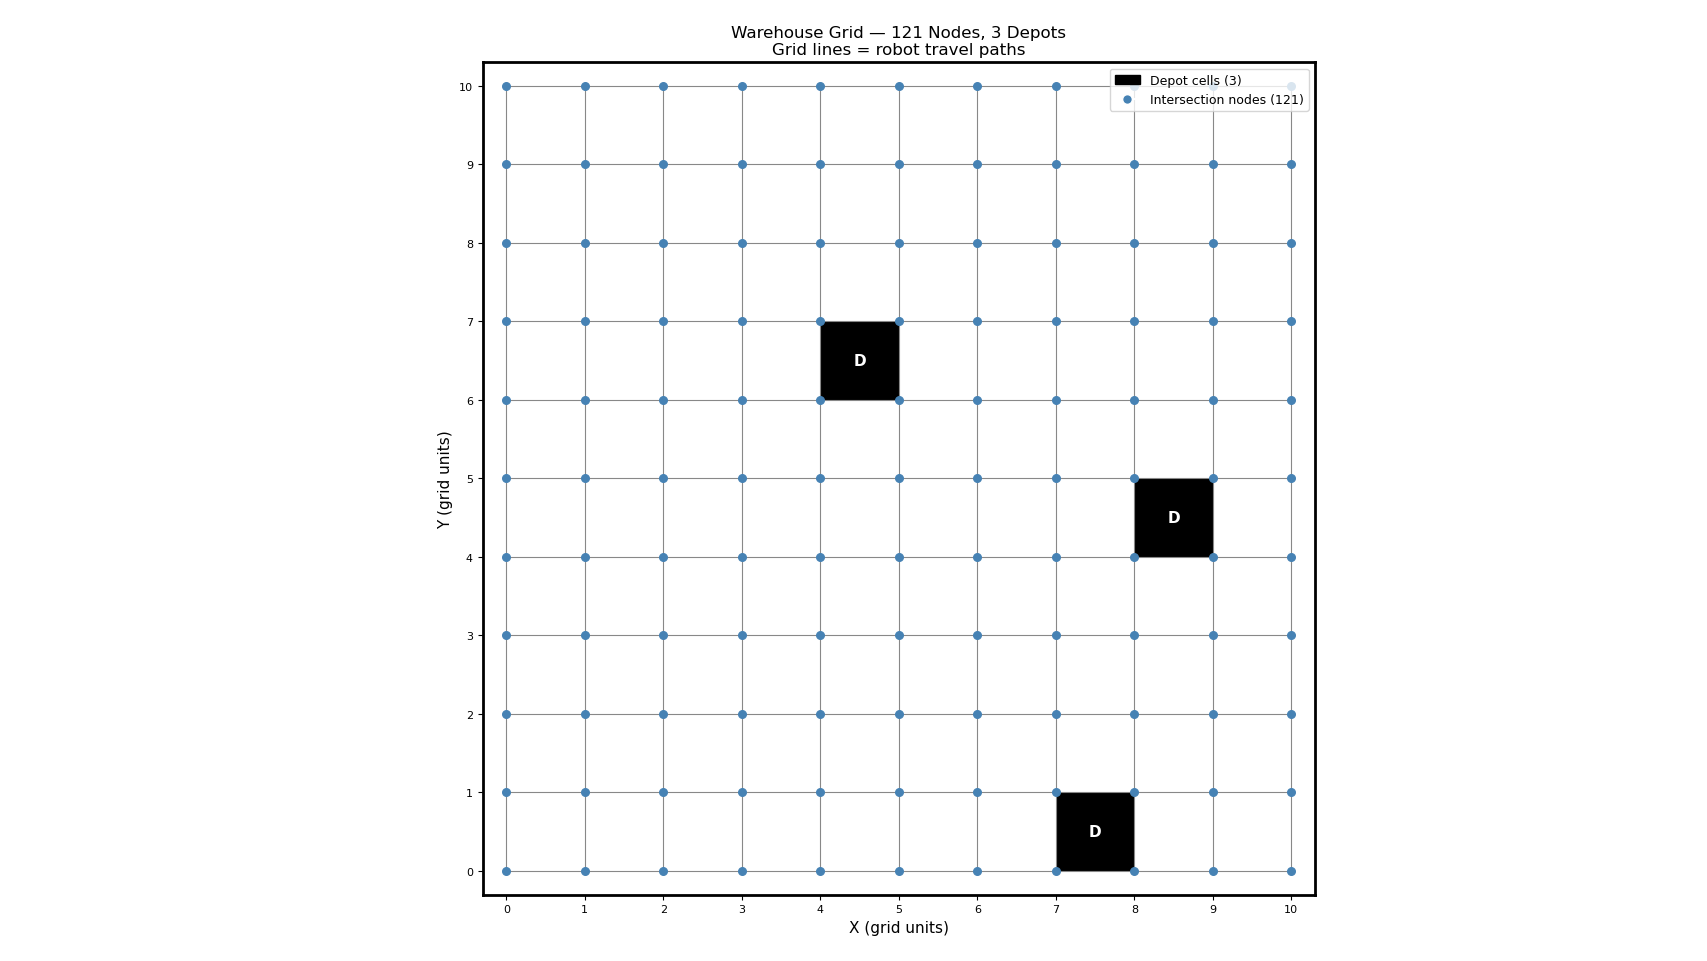
\includegraphics[width=\textwidth]{warehouse_grid_basic.png}
        \caption{Warehouse grid: 121 intersection nodes, 3 depots (black cells),
        grid edges as cobot travel paths.}
        \label{fig:grid_basic}
    \end{minipage}
    \hfill
    \begin{minipage}[t]{0.47\textwidth}
        \centering
        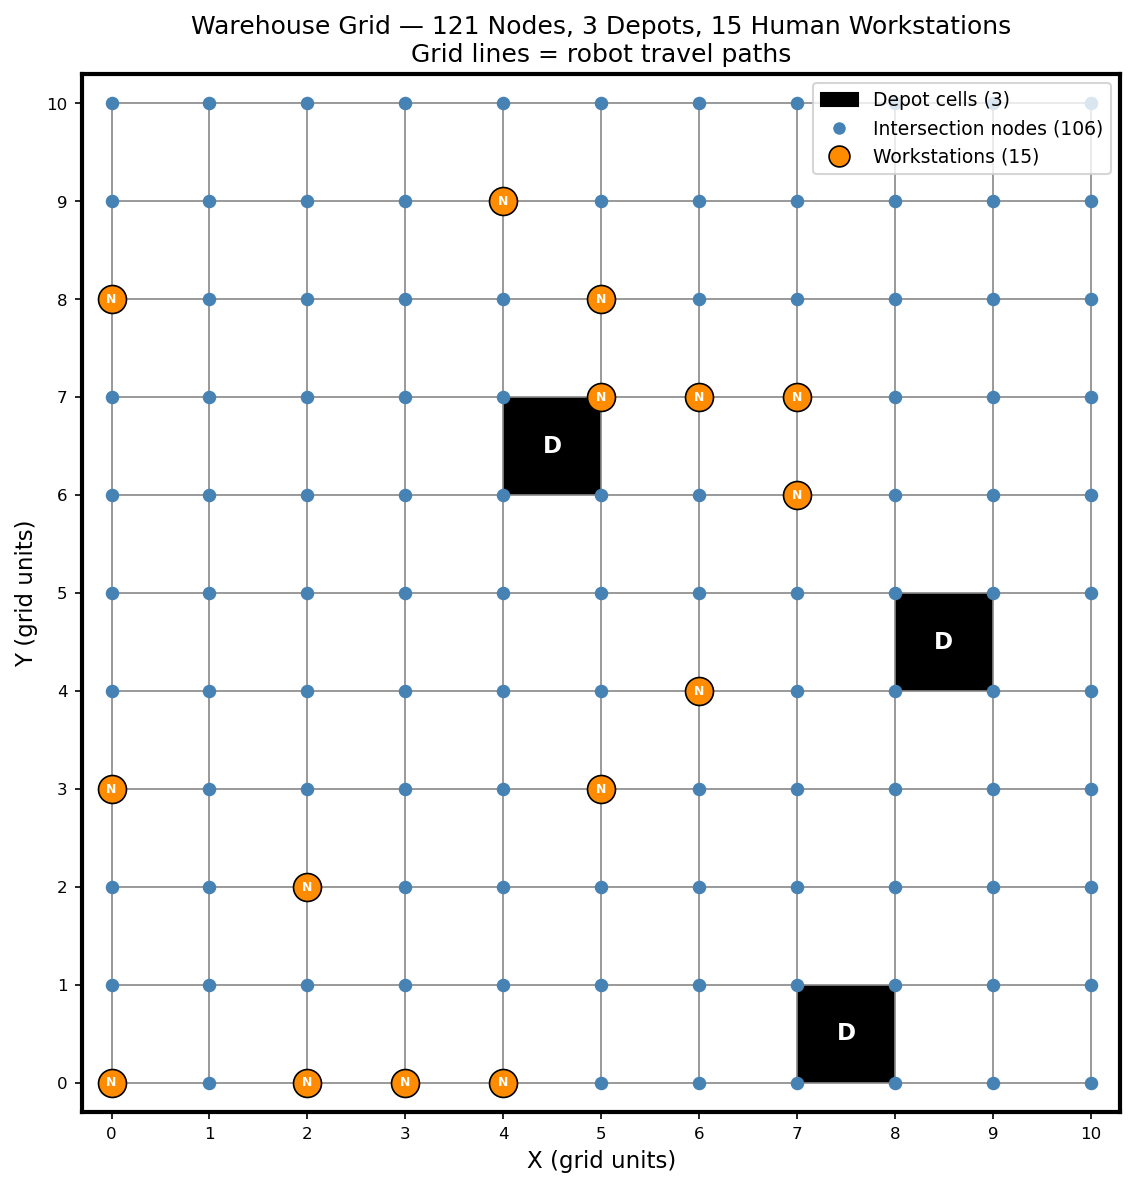
\includegraphics[width=\textwidth]{warehouse_grid_workstations.png}
        \caption{Same grid with 15 workstation nodes (orange, marked $N$) placed
        randomly across intersections.}
        \label{fig:grid_workstations}
    \end{minipage}
\end{figure}

\subsection{Extended VRP-RPD}

\begin{definition}[Multi-Depot Stochastic VRP-RPD]
Given graph $G$, depot set $\mathcal{D}$, cobot fleet of size $m$ with capacity
$k$, and workstation set $W$ with processing times $\{P_j\}_{j \in W}$, find
routes for all cobots such that:
\begin{enumerate}
    \item Each cobot starts and ends at its home depot.
    \item Each workstation $j \in W$ receives exactly one dropoff and one pickup.
    \item The pickup at $j$ occurs no earlier than processing completion:
    $t_j^{\text{pick}} \geq t_j^{\text{drop}} + P_j$.
    \item Any cobot may perform the pickup at $j$, independent of which cobot
    performed the dropoff.
    \item The number of shelves carried by a cobot does not exceed $k$ at any
    point in its route.
    \item The objective is to minimize $\mathbb{E}[\max_i T_i^{\text{return}}]$,
    where $T_i^{\text{return}}$ is the time cobot $i$ returns to its home depot.
\end{enumerate}
\end{definition}

Constraint~3 enforces temporal precedence between dropoff and pickup. Constraint~4
is the cross-agent relaxation that distinguishes this formulation from classical
pickup-and-delivery problems. Constraint~5 governs the dynamic load of each
cobot, which decreases by one at each dropoff and increases by one at each
pickup.

\subsection{MAPF on the Warehouse Grid}

Given planned routes $\{\pi_i\}_{i=1}^m$ from VRP-RPD, the MAPF problem finds
time-expanded paths $\{\hat{\pi}_i\}$ such that no two cobots occupy the same
node at the same timestep, no two cobots traverse the same edge in opposite
directions at the same timestep, and no cyclic waiting dependencies exist. The
MAPF solution may insert wait actions, increasing effective edge traversal times
beyond $d_{uv}$.

\subsection{Feedback Problem}

Let $\Delta_{uv}^{(t)}$ denote the delay on edge $(u,v)$ introduced by MAPF
at iteration $t$. The effective travel time is $\hat{d}_{uv} = d_{uv} +
\Delta_{uv}^{(t)}$. When $\hat{d}_{uv} > d_{uv}$ for edges in the planned
routes, the VRP-RPD objective value changes and pickup timing constraints may
become infeasible. The feedback problem is to determine when these delays
warrant replanning and how to update travel time estimates to produce a
consistent joint solution.

% ============================================================
\section{Two-Layer Architecture}
\label{sec:method}
% ============================================================

\subsection{Overview}

The architecture iterates between a search layer and a planning layer until the
two produce a consistent, collision-free solution. Algorithm~\ref{alg:main}
states the procedure. The search layer (ALNS$\to$BRKGA) assigns tasks and
sequences routes to minimize expected makespan. The planning layer (MAPF)
resolves spatial conflicts on the warehouse grid. When MAPF detects collisions,
it identifies which route segments caused them and returns that information to
the search layer. ALNS destroys those segments and repairs them, producing
revised routes that are checked again by MAPF. The loop terminates when MAPF
finds no conflicts or a maximum iteration count is reached.

\begin{algorithm}[H]
\caption{VRP-RPD/MAPF with Critical-Path Priority}
\label{alg:main}
\begin{algorithmic}[1]
\Require Graph $G=(V,E)$, depots $\mathcal{D}$, workstations $W$,
         fleet size $m$, capacity $k$, processing distributions $\{F_j\}$,
         maximum iterations $\text{iter}_{\max}$
\Ensure Collision-free time-expanded paths $\{\hat{\pi}_i\}_{i=1}^{m}$
\State $\text{iter} \leftarrow 0$
\Repeat
    \State $\{\pi_i\},\, \{T_i\} \leftarrow \textsc{ALNS-BRKGA}(G, \mathcal{D}, W, m, k)$
    \State $i^* \leftarrow \arg\max_i\, T_i$ \Comment{agent on critical path}
    \State $\rho \leftarrow$ rank agents by $T_i$ descending; $i^*$ receives rank 1
    \State $\{\hat{\pi}_i\},\, \mathcal{C} \leftarrow \textsc{MAPF}(\{\pi_i\},\, \rho)$
    \If{$\mathcal{C} = \emptyset$}
        \State \Return $\{\hat{\pi}_i\}$
    \EndIf
    \State $\mathcal{S} \leftarrow \{(i,\,\ell) : \text{agent } i
           \text{ has a conflict on segment } \ell\}$
    \State $\{\pi_i\} \leftarrow \textsc{ALNS-Repair}(\{\pi_i\},\, \mathcal{S})$
    \State $\text{iter} \leftarrow \text{iter} + 1$
\Until{$\text{iter} = \text{iter}_{\max}$}
\State \Return $\{\hat{\pi}_i\}$
\end{algorithmic}
\end{algorithm}

\subsection{VRP-RPD Solver}

We extend the ALNS$\to$BRKGA pipeline from~\cite{vrp_rpd_gecco_2026} to the
multi-depot stochastic setting. ALNS destroy-repair operators replace
deterministic pickup timing constraints with chance constraints:
\begin{equation}
    \Pr\left(t_j^{\text{pick}} \geq t_j^{\text{drop}} + P_j\right) \geq 1 - \alpha
\end{equation}
where $\alpha$ is a service level parameter. The BRKGA chromosome is extended
to include depot assignment, enabling joint optimization of routing and depot
allocation.

\subsection{MAPF Solver}

The MAPF solver operates on a time-expanded graph in which each node is a pair
$(v, t) \in V \times \mathbb{Z}_{\geq 0}$. Given routes $\{\pi_i\}$ from the
search layer, the solver checks for vertex conflicts (two cobots at the same
node at the same timestep) and edge conflicts (two cobots traversing the same
edge in opposite directions at the same timestep).

\textbf{Priority ordering from the critical path.} Standard MAPF solvers
assign agent priorities independently of task structure. We derive the priority
ordering directly from the VRP-RPD solution. Let $T_i$ denote the completion
time of cobot $i$ in the current VRP-RPD solution. The critical agent
$i^* = \arg\max_i T_i$ determines the makespan; any delay to $i^*$
propagates directly to the objective. Cobots are ranked by $T_i$ in descending
order: the cobot with the highest completion time receives the highest priority
and never yields to a lower-ranked cobot when a conflict arises. When two
non-critical cobots conflict, the lower-ranked cobot inserts a wait step.

This ordering ensures that MAPF conflict resolution does not extend the critical
path. Delays are absorbed by cobots with slack between their own completion time
and the current makespan.

The solver outputs a time-expanded path $\hat{\pi}_i = \{(v_0, t_0), (v_1,
t_1), \ldots\}$ for each cobot $i$, including all inserted wait steps, and a
conflict set $\mathcal{C}$ identifying each unresolved conflict as a tuple
(agent $i$, segment $\ell$, timestep $t$).

\subsection{Feedback Coupling}

When MAPF returns a non-empty conflict set $\mathcal{C}$, the feedback step
identifies which route segments caused conflicts and passes them to the ALNS
repair procedure.

\textbf{Conflict localization.} Each conflict $(i, \ell, t) \in \mathcal{C}$
names a specific agent $i$ and the route segment $\ell$ on which the conflict
occurred. The feedback step constructs the destroy target set:
\begin{equation}
    \mathcal{S} = \{(i, \ell) : \exists\, t \text{ s.t. } (i, \ell, t) \in \mathcal{C}\}
\end{equation}

\textbf{ALNS destroy.} For each $(i, \ell) \in \mathcal{S}$, the ALNS destroy
operator removes segment $\ell$ from cobot $i$'s route. The tasks associated
with the removed segment are returned to an unassigned pool. Routes for cobots
not in $\mathcal{S}$ are held fixed.

\textbf{ALNS repair.} The repair operator reinserts unassigned tasks into the
partial routes. The space-time cells occupied by non-destroyed routes at each
timestep are passed to the repair operator as forbidden zones. The repair
operator selects insertions that avoid those zones, using BRKGA to score
candidate routes. Because the cross-agent relaxation allows any cobot to
retrieve a shelf regardless of which cobot delivered it, the repair operator
may reassign a task to a different cobot entirely if that avoids the conflict
region.

The repaired routes constitute the input to the next MAPF call. This loop
continues until MAPF returns $\mathcal{C} = \emptyset$ or the iteration
limit is reached.

\subsection{Processing-to-Travel Ratio}

We hypothesize that the ratio $\rho = \mu_j / \bar{d}$, where $\bar{d}$ is the
mean inter-node travel time, determines when cross-agent retrieval reduces
makespan relative to same-agent round trips. When $\rho \gg 1$, a robot
assigned the same-agent round trip waits longer than it travels, and
reassigning that wait time to additional deliveries reduces makespan. When
$\rho \approx 1$, same-agent round trips incur little idle time and the
additional coordination in cross-agent retrieval produces no gain. The crossover
value of $\rho$ is measured on the physical testbed.

% ============================================================
\section{Experiments}
\label{sec:experiments}
% ============================================================

\subsection{Physical Testbed}

\textbf{[To be completed.]} The testbed comprises 5--6 autonomous mobile cobots
on a $10 \times 10$ warehouse grid with 121 intersection nodes, multiple depots,
and 15 workstation nodes. Processing times are sampled from distributions fitted
to observed task durations.

\subsection{Benchmark Instances}

We also evaluate on synthetic grid instances varying fleet size
$m \in \{4, 6, 8, 10\}$, workstation count $|W| \in \{10, 20, 30, 50\}$,
processing-to-travel ratio $\rho \in \{1, 2, 5, 10\}$, and depot count
$|\mathcal{D}| \in \{1, 2, 3\}$.

\subsection{Baselines}

\begin{enumerate}
    \item \textbf{Same-agent round-trip (SART).} Each cobot completes the full
    delivery-wait-retrieval cycle before accepting a new assignment.
    \item \textbf{VRP-RPD without MAPF feedback.} VRP-RPD routes are executed
    without conflict resolution; collisions are resolved locally at runtime.
    \item \textbf{MAPF with greedy task assignment.} Tasks are assigned to the
    nearest available cobot; MAPF handles all routing.
    \item \textbf{Two-layer without iterative coupling.} VRP-RPD and MAPF each
    run once with no delay feedback.
\end{enumerate}

\subsection{Metrics}

The primary metric is makespan, defined as the time at which all workstations
have been served and all cobots have returned to their home depots. Secondary
metrics are cobot utilization rate, total MAPF-induced delay, and number of
feedback iterations until convergence.

% ============================================================
\section{Conclusion}
\label{sec:conclusion}
% ============================================================

We presented a two-layer architecture that integrates VRP-RPD with MAPF for
multi-cobot warehouse coordination under multiple depots and stochastic
processing times. Existing commercial systems and MAPF formulations require the
same agent to perform both delivery and retrieval of each unit~\cite{kiva_patent_2014,
ma2017lifelong}. The cross-agent relaxation in VRP-RPD decouples shelf
processing from robot availability, and the iterative feedback mechanism
maintains consistency between the planning and execution layers as
MAPF-introduced delays alter effective travel times.

Two questions remain open for the physical testbed phase. First, the crossover
value of $\rho$ at which cross-agent retrieval reduces makespan relative to
same-agent round trips has not yet been measured. Second, convergence of the
iterative coupling under realistic conflict loads has not been characterized.
Both require physical experiments, which are in progress.

\bibliographystyle{plainnat}
\bibliography{vrp_rpd_mapf}

\end{document}
